\documentclass[11pt,a4paper,notitlepage]{article}
\usepackage[utf8]{inputenc}
\usepackage[english]{babel}
\usepackage{amsmath}
%\usepackage{indentfirst}
\usepackage{amsfonts}
\usepackage{amssymb}
\usepackage{makeidx}
\usepackage{titlesec}
\usepackage{ulem}
\usepackage{graphicx}
\usepackage{caption}
\usepackage{subcaption}
\usepackage{float}
\usepackage[left=2cm,right=2cm,top=2cm,bottom=2cm]{geometry}
\usepackage{fancyvrb}
\DefineVerbatimEnvironment{code}{Verbatim}{fontsize=\small}
\DefineVerbatimEnvironment{example}{Verbatim}{fontsize=\small}

\def\TeX{{\rm T\kern-.1667em\lower.5ex\hbox{E}\kern-.125emX}}

\title{FeyPy: A Python package for visualizing and calculating nonlinear optical properties}

\author{Adam Goler \& Team Cobra\\ Washington State University\\ Nonlinear Optics Class, Spring 2014\\ adam.goler@email.wsu.edu}

\begin{document}

\maketitle

\section{Features}

FeyPy is an object-oriented Python package. The programming objective for this package was to construct a framework for visualizing complicated nonlinear optical processes using a Feynman diagram approach and then to use those visualizations to calculate useful properties of such systems, such as the overall nonlinear response of a series of molecules interactive via optical cascading. Other useful things, such as $\LaTeX$ strings and the ability to fit data to an expected nonlinear process are also implemented.

\section{Package Directory}

\begin{figure}[htb]
\centering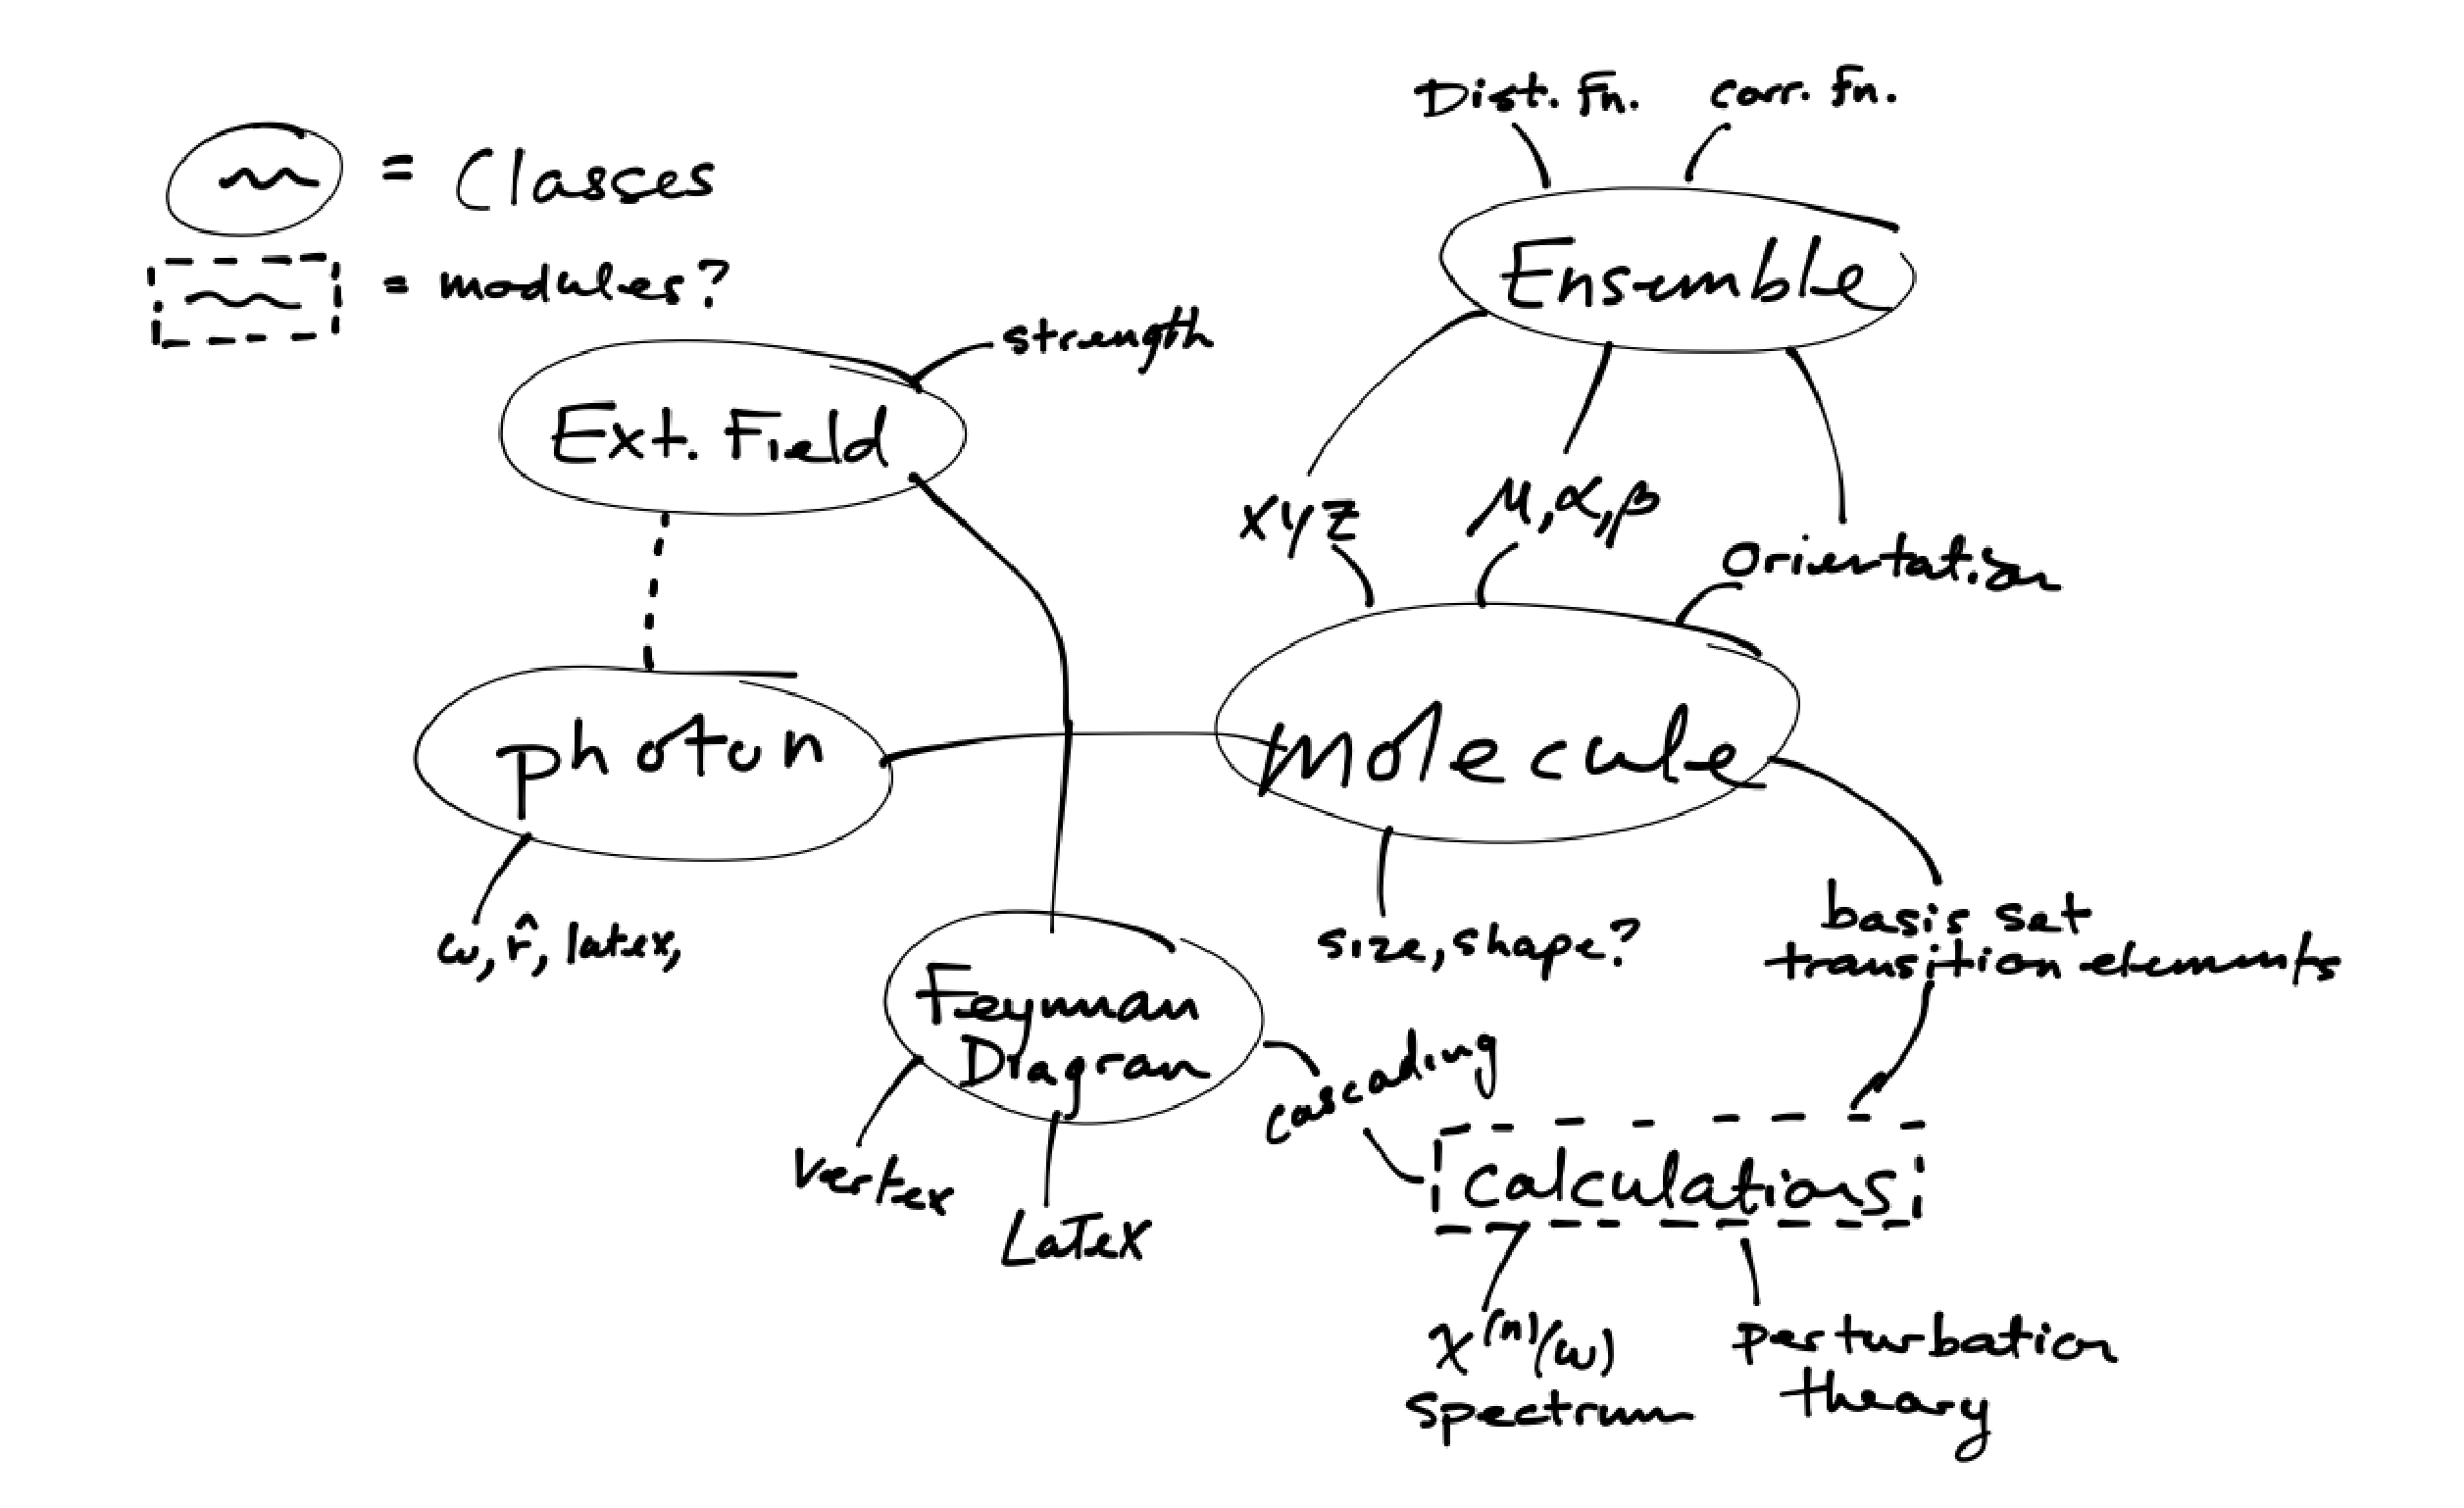
\includegraphics[scale=0.35]{bubblefig.pdf}
\caption{Hypothetical bubble chart indicating possible program structure and implied use relationships.}
\label{fig:bubblechart}
\end{figure}

\section{Getting Started}

As this packages is programmed in Python, Python is required for running any of the following calculations. FeyPy is compatible with Python v2.7 or later. In addition, Numpy 1.8 (or later) and Matplotlib is also required. 

To install FeyPy, simply download and/or extract all source code to a single directory and run with a Python interpreter. At this point, FeyPy is not configured to install directly to your Python path. Expect this to change in later iterations of the code.

The current version of FeyPy is v.0.2.

\section{Examples}

The utility of FeyPy is evidenced by its versatility. It is intended to be a one-stop-shop for visualization, calculation and fitting of nonlinear processes to the mind's eye and to experimental data. The following examples should serve as an effective introduction to the basic workings of the code. For questions about specific functions, or for a description of each available function (some are cleverly hidden to avoid accidental malarkey), see the Function Glossary (work in progress).

\subsection{Constructing a simple Feynman diagram}

Before beginning, be sure that all required packages (outlined in Getting Started) are installed. To import, make the following calls in your interpreter:

\begin{code}
from Feynman import *
from Photon import *
from Permutation import *
from Molecule import *
from CalcChi import *
from Cascade import *
# eventually, hope to have this simply be replaced with
# from FeyPy import *
import numpy as np
\end{code} 

Note any errors you receive when attempting to import the above; they could indicate improper installation of required packages. A Feynman diagram is represented by a Feynman object within FeyPy, or, alternatively, an object of class Feynman. Such an object is defined as follows:

\begin{code}
feyn = Feynman()
\end{code}

In general, there are two types of particles depicted by Feynman diagrams: photons, and molecules that are absorbing or emitting photons. Defining a single Feynman diagram (object) represents the interaction of a single molecule with an arbitrary number of photons. Within FeyPy, photons are treated as objects of the class Photon. In order to define a photon, one needs to input the frequency and polarization as basic information. (Note: Other arguments can be used when defining photons, which will be described later.)

In this example, three photons will be defined.

\begin{code}
photon1 = Photon(1,0)	# the first argument is frequency,
photon2 = Photon(1,0)	# the second argument is polarization
photon3 = Photon(-2,0)
\end{code}

To calculate meaningful results, make sure the output frequency (thus, energy) is the negative sum of the input frequencies. The polarization should be defined as either $0$, $1$, or $2$, representing photons polarized along $x$, $y$, or $z$, respectively. Units are defined such that $\hbar=1$

Once the photons are defined, all that remains is to add the photons to our Feynman diagram by using the \textit{addPhoton()} command, which takes individual photon objects as arguments. Implement as follows:

\begin{code}
# for a small number of photons, it might be easier to add individually
feyn.addPhoton(photon1)
feyn.addPhoton(photon2)
feyn.addPhoton(photon3)

# --> OR <-- for a set of photons, it may be easier to add using a for loop
photon_list = [photon1, photon2, ... photonN]
[feyn.addPhoton(photon_list[i]) for i in range(len(photon_list))]
\end{code}

This is the basic information needed to construct a Feynman diagram visualization. See the following sections for visualization methods and other calculations.

\subsection{Viewing a Feynman diagram}

Given the Feynman diagram object \textit{feyn} defined in the previous section, one may visualize the diagram with the following code:

\begin{code}
feyn.showDiagram()
\end{code}

As defined, this call results in the Feynman diagram shown in Fig.~\ref{fig:ex1} (YMMV).

\begin{figure}[h]
\centering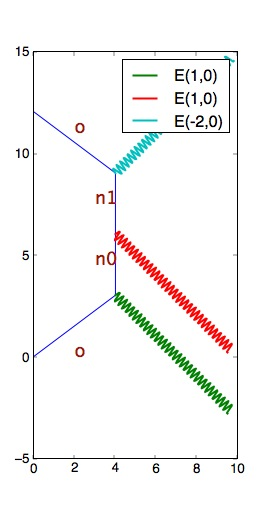
\includegraphics[scale=0.5]{feyn_example1.jpg}
\caption{Example Feynman diagram illustrating a $\chi^{2}$ nonlinear process.}
\label{fig:ex1}
\end{figure}

\subsection{Obtaining $\LaTeX$ code for a Feynman diagram}

In addition to simple visualizations of Feynman diagrams, $\LaTeX$ code corresponding to the equation for the total nonlinear response can be retrieved either as plain text or shown using Matplotlib. In order to return the plain text code, simply use

\begin{code}
feyn.getLaTeX()	# return TeX code as plain text
# returns: '\\chi^{2}=\\sum_{all}\\frac{\\mu^{0}_{gn_1}\\mu^{0}_{n_1n_0}
# \\mu^{0}_{n_0g}}{(\\Omega_{n_{0}g}-\\omega_{1})(\\Omega_{n_{1}g}-2\\omega_{1})}'
\end{code}

which, when copy/pasted into your favorite $\LaTeX$ editor (and with the removal of extra errant backslashes), results in Eq.~\ref{eq:eq_ex1}

\begin{equation}
\chi^{(2)}=\sum_{all}\frac{\mu^{0}_{gn_1}\mu^{0}_{n_1n_0}\mu^{0}_{n_0g}}{(\Omega_{n_{0}g}-\omega_{1})(\Omega_{n_{1}g}-2\omega_{1})}
\label{eq:eq_ex1}
\end{equation}

It is also possible to view Eq.~\ref{eq:eq_ex1} without the use of a $\LaTeX$ compiler within the context of the \textit{showDiagram()} command as follows:

\begin{code}
feyn.showDiagram(latex=True)
\end{code}

\subsection{Finding permutations of a Feynman diagram}

The single diagram defined previously is not the whole story. Eq.~\ref{eq:eq_ex1} refers to a sum over potentially many Feynman diagrams, which represent unique permutations of the input/output photons so defined. FeyPy can not only determine what these unique permutations are, but it can also generate Feynman objects for each permutation which can themselves be interacted with using any method defined for Feynman objects. 

To generate these permuted Feynman diagrams, use the following code:

\begin{code}
list_of_feynmans = feyn.getPermutedFeynmans() 
\end{code}

Each element of the defined list is itself a Feynman object, so each can be asked to generate an independent Feynman diagram, as shown in Fig.~\ref{fig:ex1_permutations}.


\begin{figure}[htb]
\centering
\begin{subfigure}{.33\textwidth}
  \centering
  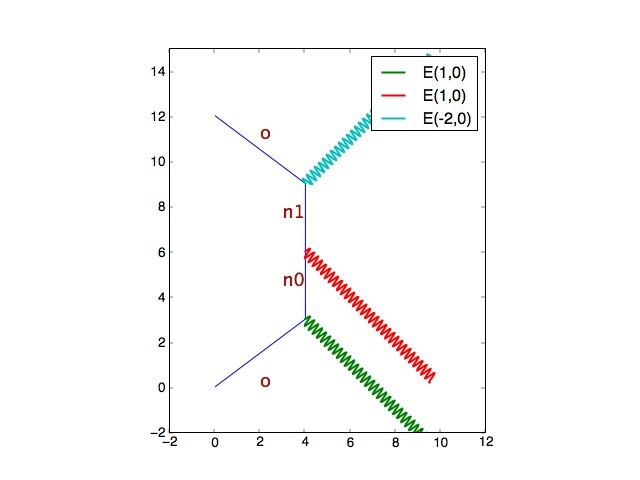
\includegraphics[width=1\linewidth]{feyn_ex1a.jpg}
%  \caption{A subfigure}
  \label{fig:sub1}
\end{subfigure}%
\begin{subfigure}{.33\textwidth}
  \centering
  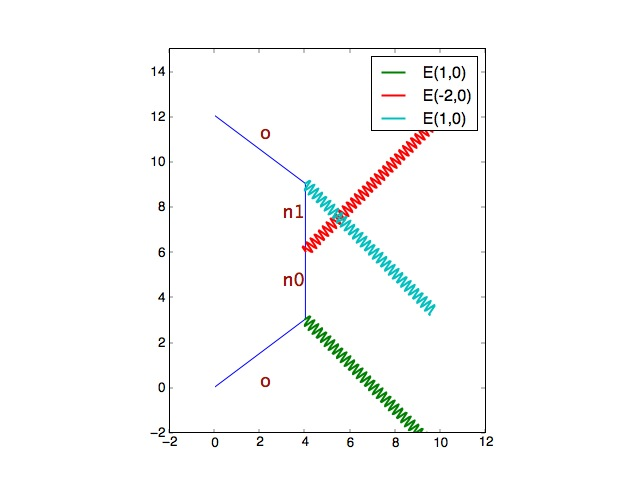
\includegraphics[width=1\linewidth]{feyn_ex1b.jpg}
 % \caption{A subfigure}
  \label{fig:sub2}
\end{subfigure}
\begin{subfigure}{.33\textwidth}
  \centering
  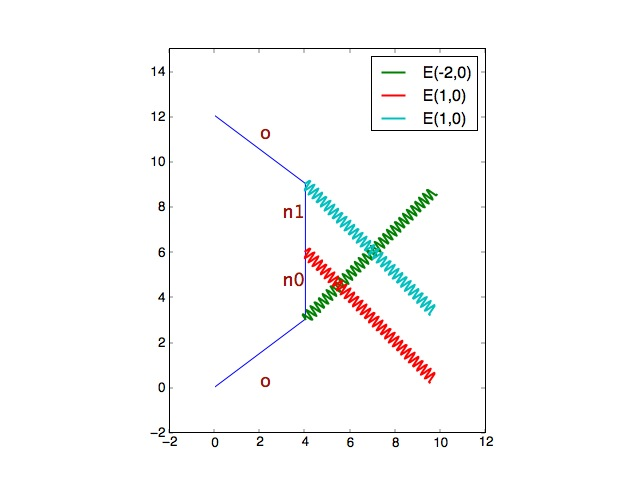
\includegraphics[width=1\linewidth]{feyn_ex1c.jpg}
 % \caption{A subfigure}
  \label{fig:sub3}
\end{subfigure}
\caption{All unique permutations of the example Feynman diagram.}
\label{fig:ex1_permutations}
\end{figure}

\subsection{Calculating the nonlinear response for a single diagram and its permutations}

Beyond the utility of visualizing Feynman diagrams, FeyPy is also capable of calculating nonlinear susceptibilities of individual diagrams or even the total nonlinearity of a set of all possible Feynman diagrams. For the Feynman object already defined as a result of the previous examples, we must first define a set of transition elements (Mu's) and resonant frequencies (Omega's) in order to calculate the nonlinear response. We use the \textit{Molecule} class to achieve this. Objects of class Molecule represent molecules who's interaction with photons are represented by Feynman diagrams (and hence Feynman objects). Besides transition elements, and transition energies, molecule objects also contain position and orientation information relative to the lab frame. This information is necessary for cascading calculations, which will be addressed later. When dealing with single molecules, position and orientation is irrelevant.

\begin{code}
molecule = Molecule()	# make a new molecule

mu = np.array([[[0, 1, 2],	# define mu's
                [1, 2, 3],
                [2, 3, 4]],
               
               [[0, 1, 2],
                [1, 2, 3],
                [2, 3, 4]],
               
               [[0, 1, 2],
                [1, 2, 3],
                [2, 3, 4]]])

molecule.setMu(mu)		# set molecule Mu matrix to mu

molecule.addOmega([1.5,2.5])	# add transition energies
					# to molecule
					# (add either individually, or
					# as a list)

feyn.linkMolecule(molecule)	# link molecule and feyn objects
\end{code}

Now we can calculate the nonlinear response of an individual Feynman object.

\begin{code}
a_chi = feyn.getChi()	# individual response
\end{code}

Or, we can calculate the total nonlinearity for the given system by adding the contributions from each possible Feynman diagram using this function

\begin{code}
a_chi = feyn.getTotalChi()	# from all permutations
\end{code}

%\begin{code}
%total_chi = 0.0	# dummy total variable
%N_diagrams = len(list_of_feynmans)	# total number of possible unique Feynman diagrams
%
%for i in range(N_diagrams):
%	total_chi += list_of_feynmans[i].getChi()
%\end{code}

Another useful feature is the ability to define a photon object as a \textit{spectrum} photon, whereas previously photons were only defined as having a fixed frequency. A spectrum photon as an input into a Feynman diagram allows for the calculation of a spectrum of $\chi$ values, i.e. a $\chi$ vs. $\omega$ plot, for example.

Following the examples laid out previously, but changing the definition of photon1 to the following:

\begin{code}
# defining spectrum frequency photons
photon1 = Photon(1,0,spectrum=True,stepfreq=0.01,startfreq=0.0,endfreq=10.0)
\end{code}

Following the previous steps aside from this minor deviation, the individual (and total) nonlinearity can also be calculated in an analogous way. Note that the \textit{getChi()} method is versatile enough to function with either a spectrum or fixed frequency photon, except that now two results are returned. (Note: Only define a single photon as a spectrum photon.) The results of this calculation are shown in Fig.~\ref{fig:chi_spec}. Currently, there is nothing to prevent the code from inadvertently dividing by zero. This issue needs to be addressed in the future.

\begin{code}
wlist,chi = feyn.getChi()	# wlist, chi, are the spectrum and chi, respectively 
showChiSpectrum(wlist,chi)	# plotting command
\end{code}


\begin{figure}[h]
\centering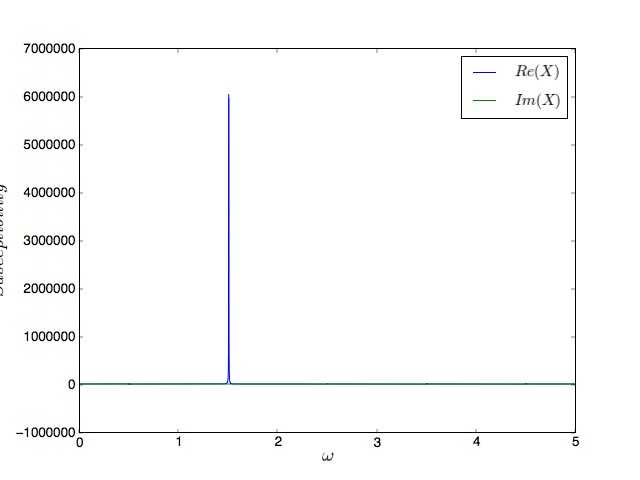
\includegraphics[scale=0.5]{chi_spectrum_fix.jpg}
\caption{Example $\chi^{(2)}$ spectrum for the aforementioned nonlinear process.}
\label{fig:chi_spec}
\end{figure}

The same can be done for the permutations of the Feynman diagram

\begin{code}
wlist,chi = feyn.getTotalChi()	# wlist, chi, are the spectrum and chi, respectively 
showChiSpectrum(wlist,chi)	# plotting command
\end{code}
 which in this case results in the same spectrum as shown in Fig.~\ref{fig:chi_spec}.

\subsection{Cascading between multiple Feynman diagrams}

The bread and butter of FeyPy is its ability to represent nonlinear cascading processes, calculate individual or total nonlinear responses, and return $\LaTeX$ strings corresponding to $\chi^{(n)}$, etc. To cascade two diagrams, a second Feynman object must first be defined, in addition to an object of class Cascade. Both Feynman objects must then be added to the Cascade object, which actually handles cascading processes.

\begin{code}
feyn2 = Feynman()	# new Feynman object
photon4 = Photon(1,0)	# new photons for feyn2
photon5 = Photon(1,0)
photon6 = Photon(-2,0)

feyn2.addPhoton(photon4)	# add new photons to feyn2
feyn2.addPhoton(photon5)
feyn2.addPhoton(photon6)

photon5.toggleVirtual()		# set photon5 to be a virtual

feyn2.linkMolecule(molecule)	# link to first molecule
						# for convenience
\end{code}

Feel free to check the appearance of \textit{feyn2}. It should be appear to be identical to our first Feynman diagram. The two diagrams can be cascaded as follows:

\begin{code}
cascade = Cascade()	# create Cascade object

cascade.addFeynman(feyn)	# add feynman diagrams
cascade.addFeynman(feyn2)	# to cascade

cascade.showDiagram()	# show cascaded diagram
\end{code}

This results in the diagram shown in Fig.~\ref{fig:casc_ex}.

\begin{figure}[h]
\centering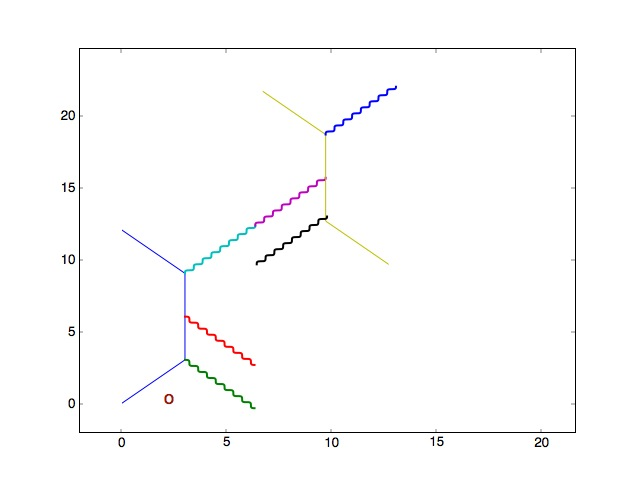
\includegraphics[scale=0.5]{cascading_ex4.jpg}
\caption{Example of a cascading process.}
\label{fig:casc_ex}
\end{figure}

\pagebreak

\section{Known Issues}

Have you had a problem with the code? Did it give output that appears wonky or inconsistent? Did you receive a strange error that you don't understand? Did your computer explode? Let us know, particularly (1) what you were trying to do (i.e. \textit{exactly} what you did), (2) what you expected to happen, and (3) what actually happened. Bonus points for screenshots or verbatim text of the error you receive, in addition to system specifications and how you are running the code. Please send all bugs to the email listed below the title of this document, adamgoler@email.wsu.edu. Thanks!

\section{Feature Request}

Do you have an idea to improve FeyPy? By all means, we'd love to hear it! Please send all requests to the email listed below the title of this document, adamgoler@email.wsu.edu. Thanks!

\begin{itemize}
	\item If one of the molecules emits two photons, is there a way to assign the one of choice for cascading?  I assume you could just use photonX.toggleVirtual() for the output photon too.  Also, what if there are two or more virtual photons exchanged? -Kuzyk
	
\end{itemize}

\section{Code Glossary}

Continually updating...

\end{document}
